\section{Research Overview}
\label{sec:overview}


Social engineering attacks on the internet can range from fully automated schemes to those involving real-time, adaptive communication by human adversaries. In this proposal, we focus on the latter, which we refer to as \textbf{Interactive Social Engineering (ISE) attacks}. These attacks involve scammers who exert sustained, interactive control over victims through multi-platform, real-time communication. Switching between communication channels is often used deliberately to avoid detection and maintain the victim's engagement. In contrast to traditional, non-interactive vectors such as phishing websites, where the static, predefined attack content is relatively easy to collect, ISE attacks rely on high degrees of human interactivity, making real-world data collection particularly challenging. This scarcity of representative datasets has, in turn, contributed to a significant gap in development of practical defenses against ISE threats. We now discuss two major representative examples to characterize these attacks.

%These scams coax victims to call fake technical support centers via various methods such as malicious advertisements, search engine poisioning, phishing emails and robocalls. Upon calling, victims who are usually targeted to be older adults are directed to share their screens under the pretext of debugging various technical support issues such as software or hardware configuration, malware mitigation. While there are many ways criminals can monetize the scam from this point, one popular method is convince the victims during these screen sharing sessions into paying for an annual support product. Unfortunatley, this is a fake-av malware that can ``freeze'' victims' operating systems on-demand and display a tech support number to initiate calls from vicitms on demand. This acts as a second entry point for a follow-up more grievous social engineering attempt by the criminals in which they transfer funds from victims' bank accounts in real-time in what is referred to as a ``Refund scam''. It is to be noted that in 2025 alone, tech-support scams account for more than a billion dollars of lost funds in the US according to the FBI's Internet Crime Complaint Center (IC3) Annual Report~\cite{}. 
\BfPara{Tech-support scams} Tech-support scams coax victims into calling fake technical support centers through various methods such as malicious advertisements~\cite{seacma,MiramirkhaniSN16}, search engine poisoning~\cite{SrinivasanKMANA18}, phishing emails~\cite{tasr}, and robocalls~\cite{PrasadDRR23}. Upon being persuaded to call, victims, who are typically older adults, are given real-time instructions to install remote desktop sharing software and share their screens under the pretext of debugging technical issues such as software or hardware configuration or malware mitigation. While there are many ways criminals can monetize the scam from this point, a common method involves convincing victims during the screen-sharing session to pay for an annual support product. Unfortunately, this product is actually fake antivirus malware that can ``freeze'' victims' operating systems on demand and display a tech support number to prompt further calls. This serves as a second entry point for a follow-up, more grievous social engineering attack, during which criminals manipulate victims into transferring funds from their bank accounts in real time—an attack referred to as a refund scam~\cite{tasr}.
% ABOVE ADD ANOTHER CITE TO YOUTUBE VIDEO.
This intentional transfer of funds allows criminals to bypass defenses such as multi-factor authentication, which are pervasively deployed in modern-day web applications and would otherwise require compromising an additional device such as the victim's phone. In 2024 alone, tech-support scams resulted in over \$1.4 billion in reported losses in the U.S., according to the FBI's Internet Crime Complaint Center (IC3)~\cite{ic3_report_24}. Reported losses from these scams rose by 14\% in 2023 and 58\% in 2024, underscoring the growing severity of the threat. Since many victims are unaware they have been targeted, this figure likely underrepresents the true scale of financial harm. Given the substantial economic impact of these scams and the intricate interactions they involve, we treat tech-support scams as a canonical form of ISE attacks and designate them as one of the primary focal points for defense in this project.
\todo{Add cite for how long this has been going on. I remember this being mentioned during Dubai trip (2012??)}


%Furthermore, these reported losses increased by 14\% and 58\% in 2023 and 2024 respectively, indicating the growing seriousness of this issue. Given that many victims of these attacks remain unaware of their incidence, this figure represents only a conservative estimate, highlighting the extent of financial damage potentially caused by these scams. Given the significant monetary losses caused by this scam and the complex interaction modes between scammers and victims, we consider tech-support scams a prominent example of ISE attacks and make it one of our main targets for defense in this project.


% NOTE TO ME (PHANI)
% I WANT TO CITE PROSPER PAPER BELOW -- BUT IT WEAKENS THE NARRATIVE ABOUT TOTAL COSTS OF THE ATTACKS.
% SO, I WILL SKIP THAT.
% NOTE TO ME (PHANI)
\BfPara{Cryptocurrency credential theft} Another upcoming example of ISE attacks is in the domain of cryptocurrencies. Recently, the PI uncovered the widespread nature of interactive scams on social media platforms, where scammers impersonate cryptocurrency exchanges~\cite{honeytweets}. These attackers exploit social media APIs on X to automate initial contact with potential victims. Subsequently, they steer victims to scammer-in-the-loop conversations on other platforms such as Instagram, Telegram or e-mail. This cross-platform handoff prevents any single platform from gaining end-to-end visibility into the scam, thereby thwarting remedial actions. Using real-time social engineering tactics, the attackers ultimately persuade victims to reveal key phrases associated with their cryptocurrency wallets. The study documented over \$1 million USD in Bitcoin stolen through these methods.
%Both US-based government agencies and cryptocurrency platforms cited similar attacks happening via telephony channel as well in which victims are directed to open their web browser and visit tailored phishing sites in their web browsers ~\cite{ic3_crypto_psa,coinbase_psa}. 
%Both U.S.-based government agencies and cryptocurrency platforms have reported similar. 
More dangerously, ISE attacks occurring via telephony channels are also reported, where scammers social engineer the victims into giving up their cryptocurrency wallet credentials~\cite{coinbase_psa,ic3_crypto_psa} leading to immediate and irreversible monetary losses. This is unlike traditional password-stealing phishing attacks where attackers still need to devise post-attack monetization strategies for the stolen data. 
%%% [CANDIDATE FOR REMOVAL] BELOW CAN BE REMOVED?
It is worth noting that, beyond ISE-based credential theft, the cryptocurrency space is also plagued by several other fraudulent schemes such as pump-and-dump operations~\cite{XuL19}, fake giveaways~\cite{LiLG23,0001KMISTTVM24,LiYN23} and investment scams~\cite{SiuH23,SiuHV022,VasekM15}, as well as adapted versions of DNS-related threats like domain dropcatching~\cite{MuzammilWBN24} and typosquatting~\cite{MuzammilWHKN24}. However, despite this wide range of cryptocurrency scams, the FBI's IC3~\cite{ic3_report_24} report highlights that cryptocurrency credential loss alone resulted in over \$1.1 billion USD in losses in the U.S. in 2024. This underscores the significant role that ISE-based attacks are playing in driving financial harm.

%It remains difficult to separate out the impact of these ISE-based attacks from many other kinds of scams plaguing the cryptocurrency realm such as giveaways via bots or streams~\cite{LiLG23,0001KMISTTVM24,LiYN23}, pump-and-dump and other investment scams~\cite{SiuH23,SiuHV022,XuL19,VasekM15}, or typosquatting fraud~\cite{MuzammilWHKN24}. However, FBI's IC3 annual report does establish the overall reported monetary loss due to  
%This multi-channel usage again makes it difficult to 

% NOTE TO ME (PHANI)
% By using multiple classes abvoe, we can go beyond the issue of this being a TSS-only project. 
% NOTE TO ME (PHANI)

%Example-1: PI's work. etc.
% I will talk about this in a bit may be, the fact that not much work exists in either of these cases?

%, if one were to get a representative dataset of fine-grained datasets such as the transcripts made by the scammers during the calls or the UI events being convinced to be made by the victims duirng the calls, it would be easy to both ``generate'' and ``evaluate'' detection solutions. Unfortuantely, most such data does not exist and we only have to rely on stories recounted by victims who are already under emotional trauma of real-world ``call scripts'' that scammers use when making these telephone calls, it might be reasoble to assume that it would be easy to generate a telephone call 

The substantial financial damages being incurred due to ISE attacks makes it clear that this remains an important and growing problem in today's society. As we discuss further in Section~\ref{sec:related_work}, most prior work has focused on detecting the precursors to ISE attacks such as malicious advertisement, scam websites and robocalls rather than building defenses aimed at directly detecting the content of the attack itself. We argue that the primary reason for the lack of such defenses is the absence of a real-world, representative ISE attack dataset -- a problem that we aim to address in this research. \todo{Add cites here}

As a contrasting example, we consider a well studied non-interactive social engineering attack:phishing emails that lead victims to password-stealing phishing websites. This non-interactive nature of this attack, solely comprising two static components, makes it feasible to collect large scale data. For instance, vigilant users who recognize the attack can ``report'' the email to security entities who leading to large-scale phishing databases (\eg OpenPhish, APWG and Phishtank). This exemplary attack data has in turn driven extensive academic research work aimed at analyzing~\cite{TianJ0Y018,PengXQ0VW19,OestZWNBZTDA20,crawlphish,SubramaniMSVP22,Sanchez-RolaBBB23,0004HK24,LimPK24,LeeLK0K25,LimLJ0KK25} and defending against~\cite{ZhangHC07,afroz2009phishzoo,AbdelnabiKF20,spartacus,LiHDLCOLH24} phishing websites. In addition, data sources such as the Certificate Transparency Logs have also stimulated defensive research enabling discovery of zero-day phishing websites in the wild~\cite{DrichelDBM21,KondrackiASN21,BijmansBSNW21,phishpedia,phishintention,dynaphish,phishllm,Teoh0LHD24}. This real-world attack knowledge has also fueled the design of more phishing-resistant user interfaces in both web browsers~\cite{EgelmanCH08,LinGTMA11,AkhaweF13,ThompsonSSWSF19,0002JW021} and email applications~\cite{Hu018,PetelkaZS19,cooper2021heads,YuAKWW23}. 


The key takeaway is that, while the wide availability of data has spurred significant research into non-interactive social engineering attacks, the same does not hold for ISE attacks. A cognizant victim typically disengages from the scammer as soon as they realize the deception. Even when a gullible victim maintains extended interaction, the exchange often spans multiple channels (\eg phone, desktop screen sharing) and is rarely recorded in a format suitable for reporting. As such, unlike web-based phishing where reporting is widely supported across both organizational systems and end-user products~\cite{LainKC22,KerstenBAZ22,pilavakis2023didn,MarinBZA23,doubly_dangerous}, we are not aware of any widely deployed systems that facilitate recording and reporting of ISE attack data for further analysis. Any after-the-fact reports submitted to law enforcement agencies are limited to the victims' recollections, who are often coping with the emotional distress of being targeted. These reports suffer from limited granularity and memory-related inaccuracies, making them insufficient for driving robust detection or analysis efforts.


In the absence of deliberate and systematic defense mechanisms against ISE attacks, an unlikely group has stepped in to fill the gap: independent internet vigilantes. These individuals have taken it upon themselves to engage directly with scammers, often manually baiting them in real time to waste their time or, in some cases, to expose their operations. As this is an extremely labor-intensive process, their efforts can disrupt scams only to a limited extent. However, many of these scam baiters possess deep, experience-driven knowledge of attacker behaviors and tactics. Their work offers valuable glimpses into attacker workflows, yet the insights they generate remain scattered across isolated online spaces such as forums and Discord servers where these communities coordinate their activities. Currently, this raw and unstructured knowledge remains siloed and is not being leveraged for broader defense or educational purposes. This raises a compelling question that we aim to address in this research project: \emph{Can we systematically collect, curate, and analyze the work and expertise of these underutilized scambaiting communities to build effective defenses and educational interventions against ISE attacks?}

We attempt to address this challenge with a 4-phase research project design that will be powered by the knowledge we expect to gain from online scambaiting communities. We provide an overview of this below.

%\BfPara{Thrust-1: Scambaiting community studies} In this first thrust, we plan to conduct various kinds of user studies involving scambaiting community members. Using the knowledge from this, we plan to establish a basic taxonomy of ISE attacks targeted by the scambaiting community along with their operational characteristics. Further, we expect to gain information about the procedure used by the community members about finding new ISE attacks, the hardware and software setup used by them for interactions, and their end goals for each kind of ISE attack. We are also interested in finding information about the follow-up actions taken by the scambaiter community such as the entities to whom they report this. As scambaiting might often stretch into the offensive side, we are also interested in finding more information about what actions scammers might pursue in this regard and for what objectives. We plan to utilize interview studies that help in providing wide range of data regarding the ISE attacks that baiters have experience with historically. To complement for memory issues and missing fine-grained studies, we also plan to utilize a carefully designed, IRB-approved protocol for performing a controlled observational study of live scam baiting activities by scammers. Finally, we plan to cap off these user studies with a co-design workshop where we include the baiters in designing a blueprint for a scambaiting tool to counteract various ISE attacks. We plan to supplement these in-person studies with thematic analysis of passive communication data between scambaiting participants on various software platforms that they use for communication. This data allows us access to much finer-grained information then can be gathered from limited time human studies. We will follow up this study with both a theoretical and empirical analysis of how the techniques used by the scambaiting community relate to what is known about ISE attacks from academic research. We expect this analysis to be mutually benefical to both the scambaiting communities as well as academic researchers helping close the bridge between these two groups and letting them adapt to what is better. 


\BfPara{Thrust-1: Scambaiting Community Studies}
In the first thrust of this project, we aim to study the scambaiting community through a combination of user research methods and passive data analysis. Our goal is to understand how these volunteer actors engage with and counteract ISE attacks, and how their strategies can inform broader defense efforts. To support this work, we have already received a letter of collaboration from the founder of a popular scambaiting forum with over 25,000 registered members and more than 300 weekly active participants. We plan to recruit participants from multiple such forums and then conduct interview-based user studies with experienced members of these communities. Through these interviews, we aim to construct a taxonomy of the types of ISE attacks targeted by the community members, along with associated attacker behaviors and operational characteristics. These studies will also surface insights into how scambaiters discover new scams, the hardware and software configurations they use for engaging with scammers, and their intended outcomes across different scam scenarios. 

\begin{wrapfigure}{R}{0.65\textwidth}
  \centering
  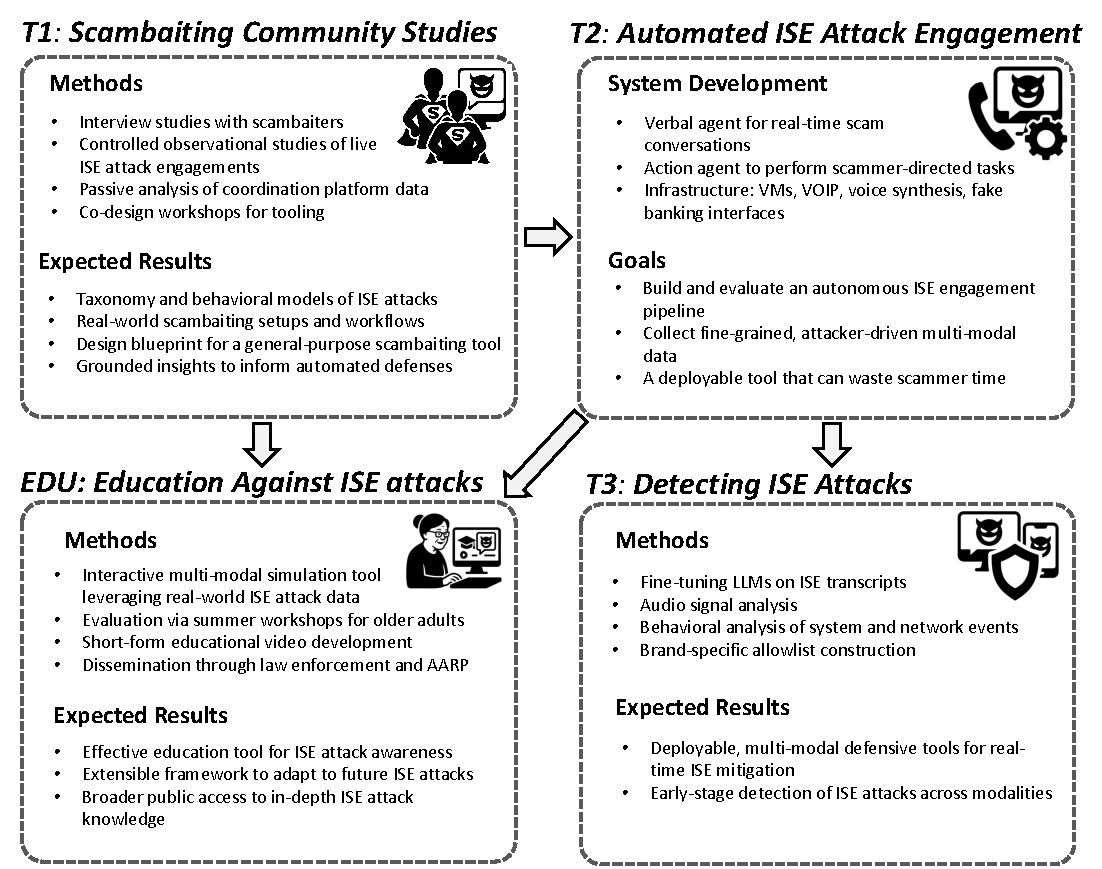
\includegraphics[width=0.63\textwidth]{images/project_overview.pdf}
  \caption{Overview of the project showing the four core thrusts: T1 (Scambaiting community studies), T2 (Automated ISE attack engagement), T3 (Detecting ISE attacks), and EDU (Education against ISE attacks). \todo{Include BI in the figure!}}
  \label{fig:project_overview}
\end{wrapfigure}
To account for recall limitations and gain more granular insights, we will complement interviews with a controlled, IRB-approved observational study of live scam baiting sessions. Additionally, we will analyze passive communication data from platforms where scambaiting communities coordinate (\eg forums, Discord). This data will provide broader and finer-grained coverage of scambaiting practices, helping to contextualize our human studies and uncover behavioral norms, technical tips, and reporting pathways. As part of the final stage in this thrust, we will conduct a co-design workshop with community members to collaboratively develop a blueprint for a general-purpose scambaiting tool. Finally, we will carry out a comparative analysis to map the techniques used by scambaiters against the academic understanding of ISE attacks. This two-way analysis will help bridge gaps between community practice and scholarly knowledge, offering mutual benefits: better-aligned defenses for the scambaiting community and more field-informed threat models for researchers.

%Our research explores how to extract, structure, and operationalize this crowdsourced knowledge to improve the broader ecosystem's resilience to ISE attacks. This research aims to bridge that gap by extracting actionable intelligence from these scattered sources and transforming it into structured datasets, threat models, and public awareness resources.

\BfPara{Thrust-2: Automated ISE Attack Engagement}
Building on insights from the scambaiting community and the observational data collected in Thrust-1, this thrust aims to design, develop, and deploy an automated pipeline capable of engaging with scammers in the wild. The system will pursue autonomous, multi-modal interactions that continue through the various stages of an ISE attack until reaching monetization. The architecture will consist of two main components: a verbal agent responsible for real-time conversation with the scammer, and an action agent that executes suggested behaviors such as enabling remote desktop access or navigating to banking websites. The system will be engineered using hardware and software components identified as practically useful by the scambaiting community. We anticipate this will include VOIP gateways, virtual machines, voice synthesizers, and replicas of financial apps and websites. Recorded calls and interaction traces from the observational studies in Thrust-1 will serve as a foundational dataset for designing, training, and evaluating this automated pipeline.

To bootstrap deployment, we will leverage both prior academic work, including the PI's research on mining ISE attack entry points in the wild~\cite{seacma,tasr,MiramirkhaniSN16,SrinivasanKMANA18,honeytweets}, and operational knowledge obtained from the scambaiting community. The system will serve dual purposes: (1) collecting fine-grained forensic and operational data about real-world ISE attack strategies, and (2) wasting scammers' time, thus acting as a direct defensive mechanism. The resulting system will generate the first large-scale dataset of attacker-driven, real-world, multi-modal ISE interactions. We are committed to upholding strong ethical standards in this thrust. One version of our study protocol, which involves live deception experiments without post-study debriefing or consent, has already been reviewed and approved by a 12-member IRB panel at our institution following extensive discussion of the legal, social, and criminological dimensions of the research.

 
\BfPara{Thrust-3: Detecting ISE Attacks}

Building on the collected real-world ISE attack datasets, this thrust focuses on developing and evaluating real-time defenses across multiple modalities, including telephony and desktop environments. These defenses will draw from the transcripts, audio content, and system-level interaction traces observed during scam engagements.

First, we will leverage parameter-efficient fine-tuning (PEFT) methods~\cite{HuSWALWWC22,DettmersPHZ23,XuXG0CZC0024} to adapt open-source large language models (LLMs) to the unique linguistic and interactional features of ISE attack transcripts derived from Thrust-2. This will enable a lightweight and practical detection pipeline capable of flagging ongoing ISE attacks as they unfold over telephony channels. A key focus will be on detecting attacks as early as possible~\cite{LiuW18,HartvigsenSKR19,RingelCFER24}, since waiting until the call progresses to a ``device compromise'' state is too late to prevent harm.

In addition to semantic signals from conversation transcripts, we will also analyze acoustic features of the audio stream. This includes both speech characteristics and background noise artifacts, which prior work has shown to be useful for mitigating malicious uses of the telephony channel~\cite{BalasubramaniyanPAHT10,KotropoulosS14,PrasadBMR20,KritsiolisK24}. Third, we will also explore detection strategies based on observed system behavior on the victims' devices. Specifically, we will study the sequence of user interface events (\eg mouse clicks, application launches) and on the victims' device and the resulting network activity that occurs either under the scammers' direction or through direct remote access.

Together, these linguistic, acoustic, and behavioral detection approaches form the foundation for a deployable defense pipeline capable of proactively identifying and interrupting ISE attacks in real time. Finally, we will construct brand-specific ISE attack allowlists by mining official contact information for commonly targeted brands identified in our earlier thrusts. These allowlists can be deployed directly by telephony carriers or endpoint devices for real-time validation and also enhance the performance of semantic detection models by serving as a reference list, following approaches used in recent work on web-based credential phishing~\cite{LiHDLCOLH24,phishintention,AbdelnabiKF20}.



% Notes: Apart from ~\cite{GuptaGBD20,BilskiJ23,RingelCFER24}, Use this link as inspiration if need be to have a "time decay factor": https://medium.com/@aditya00kumar/ranking-the-results-of-ml-models-with-a-time-decay-factor-for-large-scale-anomaly-detection-1dcf44dcd824

\BfPara{EDU: Education against ISE Attacks}
Existing educational resources for ISE attacks are typically limited to static, generic warnings that lack specificity, interactivity, and grounding in real-world scam tactics. To address this gap, we propose to develop a multimodal, interactive ISE attack simulation tool that enables users to experience realistic scam scenarios based on actual transcripts and behavioral traces collected in Thrust-2.

The tool will support branching narratives, annotations, and context-aware interactions to expose users to the multi-channel, human-in-the-loop nature of ISE attacks. We plan to design it as an extensible framework powered by generative AI, allowing us to vary instructional content and simulate diverse attack styles. We will evaluate the effectiveness of the tool through user studies conducted as part of summer workshops, with a particular focus on older adults who are especially vulnerable to these scams.

This platform will also serve as a source for generating short-form educational video walkthroughs of representative ISE attack flows. To broaden the reach of these materials, we will work with our law enforcement partners at the United States Secret Service and the local Sheriff's department to disseminate the developed videos through their community outreach and public education channels.

%a result, any after-the-fact reports submitted to agencies like the law enforcement are limited to victims' recollections, which are often insufficient for driving detection or analysis efforts due to limited granularity and memory-related inaccuracies. 


%Over the years, researchers including the PI have shown the potential for these phishing websites to also exhibit a bit of dynamicity in their content for evasive purposes which has also been studied in dept
%While we discuss a range of existing mitigatory solutions and how they fall short of combating present-day ISE attacks such as the above in Section~\ref{sec:related_work}, the financial damages being inflicted by them make it directly clear that there is a dearth of deployed solutions that neutralize their threat. Conceptually, this might be a simple problem to defend against. If one were to get a representative dataset of variuos events taking during the interactions of ISE attacks, then appropriate defensive solutions can potentially be devised based on being able to track them. 

% NOTE (TO ME): BELOW IS UNECESSARY - makes things look too simple for Thrust-3 and adds not much value.
%For example, having real-world scripts of various stories that scammers devise to direct a router configuration error into a malware issue on a user's computer that requires remote diagnosis~\cite{tasr} would be incredibly useful to devise a detection solution. Similarly, the series of specific actions performed by a victim on their computers, upon directions of the attacker (\eg opening event logger~\cite{MiramirkhaniSN16}) can also be very helpful to identify an ongoing attack. Yet, there is not much data containing real-world attacker communication so far. Unfortunately, this affects both devising as well as evaluation of any scam detection technologies. 

% NOTE-TO-SELF: IT IS BETTER TO GET RID OF THE BELOW CITATION THAN A NON-SIGNIFICANT PAPER JUST TO CONVOLUTE YOUR NARRATIVE LOGIC. KEEP IT STRAIGHTFORWARD AND TO THE POINT. 
%Instead, the limited amount of existing ISE attack defenses have relied on scripts that are artificially written by role-playing attackers~\cite{DerakhshanHB21} which does not work well given that it is driven by the scammers. 


%This project focuses on designing principled, data-driven methodologies to characterize and mitigate \emph{human-in-the-loop} social engineering attacks. In these attacks, the adversary maintains interactive control over the victims via real-time, adaptive communication them during the attack lifecycle. This can is often done via multiple platforms on multiple channels between which the attacker switches frequently as part of their strategy. We refer to these as interactive social engineering attacks (\bf{ISE}) throughout this proposal. Unlike traditional, non-interactive social engineering vectors such as phishing websites where the attack content is predefined and easy to collect, ISE attacks interactive requirements made attack data examples scarce in existence. This unfortunately led to a dearth in practical defenses for ISE attacks. 

%This project focuses on developing methodologies to study and thwart online, \emph{human-in-the-loop} social engineering attacks. Specifically, we plan to develop a multi-stage pipeline for defending against various social engineering attacks that involve interactive participation of attackers with the victims during the attack. This is in sharp contrast to non-interactive social engineering attacks such as credential phishing attacks or robocalls all of which have received significant attention from researchers until now.  ith traditional well-studied social engineering attacks such as credential phishing attacks where in the attacker only sets up a phishing website and disseminates this to the victims en masse 





-----------------------------------------------
FLOW OF THIS SECTION:

\begin{enumerate}
%\item 1. Introduce "human-in-the-loop" social engineering attacks; THe presence of "humans" makes this pretty complicated/twisty. For example, a text message from a cryptocurrency scammer will steer user to make a phone call who will then direct the user to open their computer and follow directions from there. In our recent work on crypto currency scams, we have shown the same where victims are moved from X to other platforms such as email or instagram providing additional benefits of not letting any single platform get a full-on view of the entire scam. 
%from a cryptocurrency scammer, can make the user visit

%\item 2. we present TSS scams as a representative example of this.  Owing to its complicated working nature, this will be our main focus. Money - talk about how much this alone is worth.

%\item 3. Crypto currencies are another representative example (https://www.ic3.gov/PSA/2024/PSA240801 https://www.coinbase.com/blog/hang-up-the-phone-stop-social-engineering-scams). Again money - how much is this worth overall. 

%\textbf{Note to self}: By using multiple classes, we can go beyond the issue of this being a TSS-only project. 

%\item 4. Looking back at both, if one were to get a representative dataset of fine-grained datasets such as the transcripts made by the scammers during the calls or the UI events being convinced to be made by the victims duirng the calls, it would be easy to both ``generate'' and ``evaluate'' detection solutions. Unfortuantely, most such data does not exist and we only have to rely on stories recounted by victims who are already under emotional trauma of real-world ``call scripts'' that scammers use when making these telephone calls, it might be reasoble to assume that it would be easy to generate a telephone call 

% PHANI (NOTES): MOVED THE BELOW TO T1; ITS BETTER TO SPRINKLE SOME ARGUMENTS THROUGHOUT THE PROPOSAL.
%\item 5. REGARDING SE, pretty much most of the work is on phishing in web - both measurements as well as user studies, defense etc. There's a strong reason for this. THEY HAVE LOTS OF DATA WE DON'T AND THIS MAKES IT DIFFICULT TO PURSUE DEFNESIVE MEASURES. More deeply here: In web-based credential phishing attacks, there exist a steady influx of SE attacks that are blanket-sent to everyone. Thus, they end up getting populated in blocklists. Same is not the case for human-in-the-loop attacks due to the hindrances involved in being able to gather data. natural evasive factors that disable this. As a result, most research is only using artificially generated data.   Discuss psychological factors (MOVED TO THRUST-1). 

%\item 6. Forward cite to our discussion on robocall research thus far and how it is also mainly non human-in-the-loop data driven. Better not waste too much time here as we want to talk about the main idea soon (also related work needs to have some interesting stuff too!)

%\item 7. BIG IDEA: IN THE ABSENCE OF ANY deliberate DEFENSE MECHANSISMS, a group of internet vigilantes are taking care of all this right now.  Knowledge is simply sitting in this island of isolated netowrk right now. Can we leverage this knowledge from these communities and use it to power our own defenses and educational actions? and then use it for a other boundaries? That is the main question we are trying to deal with here...

%We want to leverage them to start a 4-part pipeline for this research.


\item 8. Figure showing 4 parts (3 thrusts, 1 education)

\item 9. Thrust-1 discussion
\item 10. Thrust-2 discussion. CALLOUT ABOUT ETHICS/IRB APPROVAL ETC.
\item 11. Thrust-3 discussion.
\item 12. Edu discussion. 

\item 13. PI's past research trajectory is all devoted to realizing this big idea. In the past, focused on developing platforms for recording social engineering attacks including browser-based modification. This followed by works that used these to study web-based social engineering attacks on a large scale. These led to discovery of ecosystems involving complicated multi-channel human-in-the-loop scams with virtually no defenses other than internet vigilantes. 

\item 14. CALLOUT: THIS PI's LONG-TERM RESEARCH AGENDA IS TO WORK AGAINST THE ADAGE of "HUMAN IS THE WEAKEST LINK IN CYBERSECURITY" by developing data-driven technologies that reduce the risk as of people falling for social engineering attacks. 
REVISED (CG - ChatGPT): This PI's long-term research agenda is to challenge the prevailing adage that "humans are the weakest link in cybersecurity" by developing data-driven technologies that reduce the risk of individuals falling victim to social engineering attacks. In the context of ISE attacks, these could often be dismissed as older adults or those who are tecnologically inept to only be affected by these scams. Such a thinking is dangerous as technology should adapt to the consumers' needs and it is important to study the exact methods in which technology is being victimized.


\end{enumerate}




% -----------------------------------------------
% RANDOM NOTES FOR THIS SECTION:


% NOTES IN GENERAL:
% (1) Definitely not just TSS; baiters said they do PCH scams as well.
% (2) Perhaps, our crypto-TSS scams from SP24, or hybrid crypto-TSS (that I experienced) and ultimately, pig butchering scams all also fall under this category. 


% -----------------------------------------------

%This project focuses on developing methodologies to study and thwart victim-initiated telephony scam calls. In these scams, attackers use baits such as fake invoices or fake malware infections to ``scare'' victims into making outgoing telephone calls to the attackers. These baits are typically distributed to potential victims by abusing web search engines, online advertising networks, or email services. As only the interested victims who are already convinced by the bait make the calls, these result in ``high-quality'' opportunities for cybercriminals who then employ specialized social engineering techniques to cause real-time financial damage to them. Technical support scams, in which the attackers pretend to operate a real tech support center are a particularly problematic example of these victim-initated telephony scams. According to the FBI’s Internet Crime Complaint Center (IC3) Annual Report, U.S. victims lost over \$924 million to tech support scams in 2023 alone, with the elderly being the primary targets ~\cite{}



WHILE IN OTHER CASES, CONTEXTUAL DATA SUCH AS THE PHISHING WEBSITE, or PHISHING EMAIL or SMS can be forwarded and data can be stored, telephony conversational data is highly private - and hence detection models cannot be easily created. 



----------------
Telephony channel-based tech support scams (TSS) have become a significant societal threat, particularly targeting vulnerable populations. In these scams, cybercriminals abuse web search engines and online advertising networks to promote scam websites and persuade victims to make telephone calls to fake support centers. Figures 1 and 2 show two real world examples of TSS websites in the wild. Upon receiving calls via the phone numbers in these sites, scammers will fabricate a non-existent problem with the victims’ devices (personal computers and mobile devices), remotely connect to them, and ultimately, steal thousands of dollars as covered in many U.S. news reports [1, 2, 3]. The funds are stolen by social engineering the victims to willingly transfer the money which neutralizes any two-factor authentication (2FA) defenses that are commonly used.

According to the FBI’s Internet Crime Complaint Center (IC3) Annual Report, U.S. victims lost over \$924 million to tech support scams in 2023 alone, with the elderly being the primary targets ~\cite{}. Given that many victims of these attacks remain unaware of their incidence, this figure represents only a conservative estimate, highlighting the extent of financial damage potentially caused by these scams. Prior research, including work conducted by PI Vadrevu, has shown that this crime involves many malicious call centers operating in South Asia~\cite{}. While these call centers operate from outside the U.S., the criminals also rely on domestic money laundering networks to facilitate the illicit transfer of funds from the victims ~\cite{}. This highlights the transnational and complex nature of this crime, making it difficult to address without specialized investigative measures.

This project proposes developing multiple technologies that law enforcement agencies can utilize at scale for collecting incriminating evidence against criminals involved in tech support scam operational pipeline to aid in prosecution and mitigation efforts. As proof-of-concept, we will also deploy these technologies throughout the project period and share resulting forensic datasets with law enforcement authorities. This forms the first collection of a comprehensive tech support scam dataset with implicating information about all parties actively or passively involved in the scam pipeline. As such, this project directly aligns with Objective 4.4 to “Combat Cybercrime” in the DHS Strategic Plan for 2023-27~\cite{}. This objective is part of the department’s broader mission to secure the U.S. cyberspace. Specifically, this objective in the devised strategic plan calls for leveraging state-of-the-art cyber investigative approaches to combat cross-jurisdictional financial fraud, which is the central goal of this proposal. All the proposed tasks directly result in reusable tools, actionable insights and valuable datasets that law enforcement agencies can adopt to combat rampant tech support scams and safeguard U.S. residents.


PLAN:

Inbound telephony scams -> too much low percentage -> robocalls -> many defenses relying on data from honeypots, as well as authentication techniques. Governmental regulations also help.

Outbound telephony scams, are for some reason left out of these and are much more challenging to detect. Initiated by websites - but PI's research shows that they are not good. 

UNITL NOW NO DATA AT ALL. LITTLE WE CAN FIND IS ALL FABRICATED DATA. 


This SOK paper presents some interesting ``challenges'' that we can adapt here~\cite{TuDZA16}.


\begin{enumerate}

\item Other solutions such as STIR/SHAKN protocols mitigate the threat of inbound phone scams. [Explain how]. 
\item Works so far have also predominantly focused on reducing the threat of inbound phone scams (such as robocalls) - this is because it is more percievable.
\end{enumerate}